% =====================================================================
% ejercicio06.tex
% Responsabilidad única: documentar el diagnóstico del dataset, el
% balance de clases, la estrategia de imputación y la partición
% train/test. Los números provienen de la ejecución real del notebook
% adjunto (Taller_1_KNN_Notebook.ipynb).
% =====================================================================
\subsection{Ejercicio 6 --- Exploración inicial y preparación de datos}

\subsubsection*{a--c. Carga del dataset y diagnóstico general}

El conjunto de datos \emph{Give Me Some Credit} contiene 150.000
observaciones y 11 variables (10 predictoras más la variable objetivo
\texttt{SeriousDlqin2yrs}) de las cuales 6 son de tipo entero
[\texttt{int64}], 4 de tipo decimal [\texttt{float64}] y solo dos
presentan valores faltantes: \texttt{MonthlyIncome} (29.731 faltantes,
$19.82\%$) y \texttt{NumberOfDependents} (3.924 faltantes, $2.62\%$),
mientras que el resto de variables no tiene ningún faltante.

\subsubsection*{d. Balance de clases}

\begin{table}[H]
\centering
\begin{tabular}{lrr}
\toprule
Clase & $n$ & \% \\
\midrule
0 (no incumple) & 139.974 & 93.32 \\
1 (incumple)     &  10.026 &  6.68 \\
\bottomrule
\end{tabular}
\caption{Distribución de la variable objetivo \texttt{SeriousDlqin2yrs}.}
\end{table}

Casi 14 casos negativos por cada positivo: Un modelo trivial que
siempre prediga la clase 0 ya alcanzaría cerca de $93\%$ de Accuracy
sin ser útil en la práctica, de modo que la Precision, Recall y F1 sobre
la clase 1 serán las métricas que realmente den informen del desempeño.

\subsubsection*{e. Gráfica}

\begin{figure}[H]
    \centering
    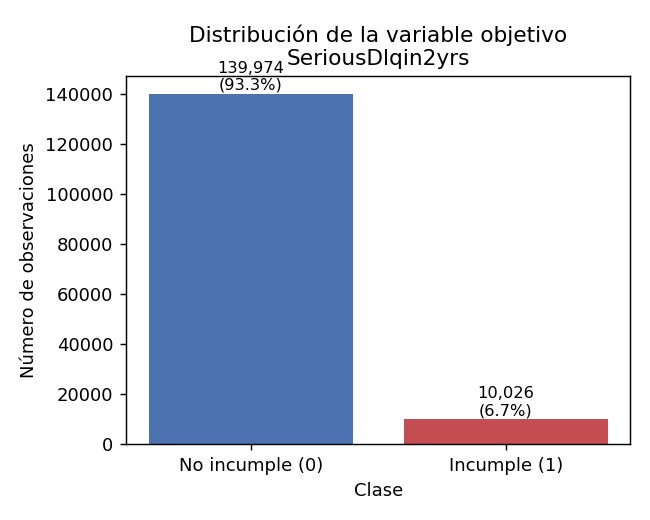
\includegraphics[width=0.55\textwidth]{figuras/ex6_distribucion_target.png}
    \caption{Distribución de la variable objetivo.}
\end{figure}

\subsubsection*{f. Tratamiento de valores faltantes}

Se imputó con la \textbf{mediana} de cada variable en lugar de la
media ya que ambas variables con faltantes tienen colas largas hacia
la derecha (unos pocos ingresos o números de dependientes
extremadamente altos que arrastrarían la media), la mediana resulta
mucho más robusta frente a esos valores atípicos, usando como
referencia \texttt{MonthlyIncome}\,$=5.400$ y
\texttt{NumberOfDependents}\,$=0$.

\subsubsection*{g. Partición 80/20 estratificada}

\begin{table}[H]
\centering
\begin{tabular}{lrrrr}
\toprule
Conjunto & Clase 0 ($n$) & Clase 0 (\%) & Clase 1 ($n$) & Clase 1 (\%) \\
\midrule
Entrenamiento (120.000) & 111.979 & 93.32 & 8.021 & 6.68 \\
Prueba (30.000)         &  27.995 & 93.32 & 2.005 & 6.68 \\
\bottomrule
\end{tabular}
\caption{Distribución de clases en entrenamiento y prueba.}
\end{table}

Se usó \texttt{train\_test\_split(X, y, test\_size=0.2, stratify=y,
random\_state=42)} (la estratificación busca mantener la proporción de
clases prácticamente idéntica entre \emph{train} y \emph{test}),
evitando que el azar de la partición produzca un subconjunto con una
tasa de incumplimiento notablemente distinta a la del conjunto
completo (lo cual sesgaría la evaluación).
